\section{Results}
\begin{figure}[h]
\hspace{-2.8cm}
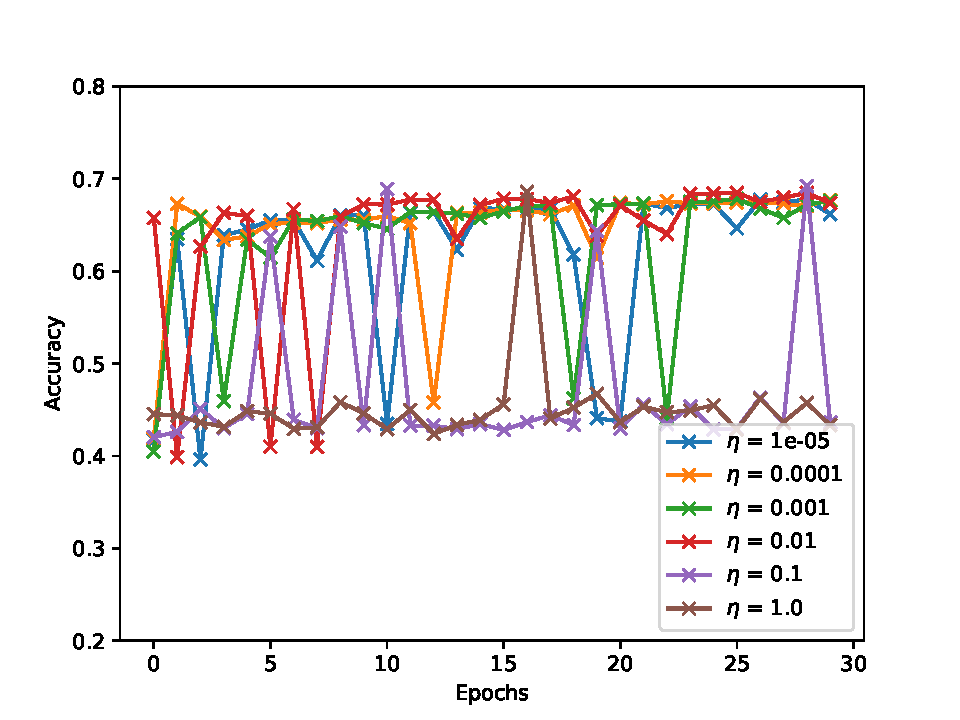
\includegraphics[width = \paperwidth]{figures/logistic_eta.pdf}
    \caption{Accuracies for a selection of learning rates $\eta$ as a function of epochs. 
    30 epochs, batch size $= 100$, and momentum parameter $\gamma = 0.01$. The accuracy
    values are measured on the test set.
    The ratio of amount of training data to test data is $0.8$.}
\label{fig:logistic-eta}
\end{figure}

\begin{table}[h]
\begin{tabular}{l|c|c|c}
$\eta$ & Training & Test & Critical  \\
\hline
$10^{-5}$ & $0.718$ & $0.680$ & $0.616$ \\
$10^{-4}$ & $0.723$ & $0.683$ & $0.624$ \\
$10^{-3}$ & $0.723$ & $0.685$ & $0.628$ \\
$10^{-2}$ & $0.712$ & $0.672$ & $0.604$ \\
$10^{-1}$ & $0.462$ & $0.430$ & $0.460$ \\
$1$    & $0.465$ & $0.446$ & $0.480$
\end{tabular}
    \caption{Accuracies for a selection of learning rates $\eta$ after 
    30 epochs. Batch size $= 100$, and momentum parameter $\gamma = 0.01$.
    The ratio of amount of training data to test data is $0.8$}
    \label{tab:logistic-critical}
\end{table}
